% Autor: Simon May
% Datum: 2017-10-05
% Diese Datei bietet ein minimalistisches Grundgerüst für ein LaTeX-Dokument,
% z.B. für die Bearbeitung der Aufgaben.
\documentclass[
	% Papierformat
	a4paper,
	% Schriftgröße (beliebige Größen mit „fontsize=Xpt“)
	12pt,
	% Schreibt die Papiergröße korrekt ins Ausgabedokument
	pagesize,
	% Sprache für z.B. Babel
	ngerman
]{scrartcl}

% Achtung: Die Reihenfolge der Pakete kann (leider) wichtig sein!
% Insbesondere sollten (so wie hier) babel, fontenc und inputenc (in dieser
% Reihenfolge) als Erstes und hyperref und cleveref (Reihenfolge auch hier
% beachten) als Letztes geladen werden!

% Silbentrennung etc.; Sprache wird durch Option bei \documentclass festgelegt
\usepackage{babel}
% Verwendung der Zeichentabelle T1 (Sonderzeichen etc.)
\usepackage[T1]{fontenc}
% Legt die Zeichenkodierung der Eingabedatei fest, z.B. UTF-8
\usepackage[utf8]{inputenc}
% Schriftart
\usepackage{lmodern}
% Zusätzliche Sonderzeichen
\usepackage{textcomp}

% Mathepaket (intlimits: Grenzen über/unter Integralzeichen)
\usepackage[intlimits]{amsmath}
% Ermöglicht die Nutzung von \SI{Zahl}{Einheit} u.a.
\usepackage{siunitx}
% Zum flexiblen Einbinden von Grafiken (\includegraphics)
\usepackage{graphicx}
% Abbildungen im Fließtext
\usepackage{wrapfig}
% Abbildungen nebeneinander (subfigure, subtable)
\usepackage{subcaption}
% Funktionen für Anführungszeichen
\usepackage{csquotes}
% Zitieren, Bibliographie
\usepackage{biblatex}


% Verlinkt Textstellen im PDF-Dokument
\usepackage[unicode]{hyperref}
% "Schlaue" Referenzen (nach hyperref laden!)
\usepackage{cleveref}

% siunitx: Deutsche Ausgabe, Messfehler getrennt mit ± ausgeben
\sisetup{
	locale=DE,
	separate-uncertainty
}

\begin{document}
\begin{titlepage}
	\centering
	{\scshape\LARGE Versuchsbericht zu \par}
	\vspace{1cm}
	{\scshape\huge E4\par}
	\vspace{2.5cm}
	{\LARGE Gruppe 2 Mo\par}
	\vspace{0.5cm}
	{\large Nils Kulawiak (E-Mail: n\_kula01@wwu.de) \par}
	{\large Oliver Brune (E-Mail: o\_brun02@wwu.de) \par}
	\vfill
	durchgeführt am 15.1.2017\par
	
	\vfill

	{\large \today\par}
\end{titlepage}


\tableofcontents
	
	
\newpage
\section{Kurzfassung}
In diesem Versuch werden Phasenübergänge von einer Cu$_{3}$Au-Legierung unter Variation der Temperatur betrachtet. Im ersten Teil des Versuchs wird das mithilfe des Debye-Scherrer Verfahrens getan. Dabei wird eine polykristalline Probe mit monochromatischer Röntgenstrahlung unter Variation des Drehwinkels bestrahlt. Ziel bei dieser Untersuchung ist es, die Gitterkonstante $a$ des fcc-Gitters zu bestimmen und ihre lineare Abhängigkeit von der Temperatur zu überprüfen. Außerdem soll untersucht werden, ob die Kernaussagen, die Debye mathematisch hergeleitet hat, auch experimentell bestätigt werden können.

Außerdem wird überprüft, inwiefern das JMAK-Modell mit experimentellen Untersuchungen übereinstimmt, insbesondere ob der Avrami-Exponent als $n=4$ angenommen werden kann. Hierzu wurden zwei verschiedene Untersuchungen durchgeführt.

Zum einen wurde der Ordnungsparameter während der Phasenumwandlung bei etwa 375°C bestimmt. Der Phasenübergang findet von hoher Temperatur bzw. hoher Unordnung zu kleiner Temperatur bzw. hoher Ordnung statt. Dabei wird die Dynamik beim Phasenübergang bestimmt und untersucht, mit welcher Potenz sich die Ordnung im Verlauf der Zeit ausbildet. Die Potenz entspricht hier gerade dem Avrami-Exponenten. Allerdings wurde ein Ergebnis gefunden, welches den theoretischen Vorhersagen nicht entspricht, sodass hier verschiedene Probleme diskutiert werden, die diese Differenz erklären.

Zum anderen wurde der Phasenübergang der Legierung mithilfe eines Kalorimeters untersucht. Hier wurde der Wärmefluss der Probe im Vergleich zum Wärmefluss einer Referenz gemessen. In einem Diagramm, in dem der Wärmefluss gegen die Zeit aufgetragen ist, kann an die Messwerte die zeitliche Ableitung der JMAK-Gleichung angefittet werden. Der hieraus bestimmte Wert ($n=3,84\pm0,02$) liegt zwar in der korrekten Größenordnung, der vorhergesagte Wert von $n=4$ liegt allerdings nicht im Intervall der Standardabweichung. Dies wird anschließend diskutiert.


\section{Interferenz von Röntgenstrahlen unter Erhöhung der Temperatur}
\subsection{Methoden und Durchführung}
Um zu gewährleisten, dass eine Wärmebehandlung während der Röntgenuntersuchung stattfinden kann, wird die Cu$_{3}$Au Probe in Scheiben geschnitten und mit einem Loch versehen, in das das Thermoelement aufgenommen wird. Diese Probe wird dann in ein mit einer Heizkammer kombiniertes Röntgendiffraktometer gegeben. Um die Oxidation der Probe zu verhindern, muss ein Vakuum erzeugt werden. Das bedeutet, dass die Messungen bei einem Druck von $10^{-15}$bar ausgeführt werden. Diese Probe wird daraufhin mit monochromatischer Röntgenstrahlung der Länge $\lambda = \SI{1,54}{\angstrom}$ bestrahlt. Gleichzeitig werden sowohl Quelle als auch Detektor gedreht, was zu einer 2$\theta$ Geometrie führt, gezeigt in \cref{theta}.

\begin{figure}[h]
	\centering
	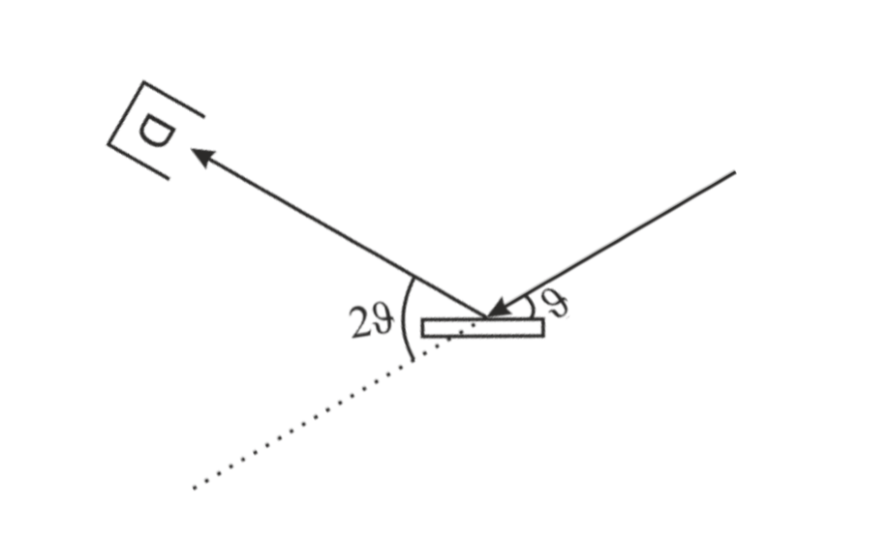
\includegraphics[scale=0.3]{2theta.PNG}
	\caption{Skizze des Versuchaufbaus}
	\label{theta}
\end{figure}

Die Intensität wird dann in 2$\theta$ = 0,02° Schritten im Winkelbereich von 20° bis 90° gemessen. Das passiert bei den Temperaturen 25°C,400°C,500°C und 700°C. Die Messdauer pro Schritt beträgt 0,5s. Da es bei der 700°C Messung zu Komplikationen kam, wurde dort in 0,04° Abständen gemessen und die Messung ist bei 80,52° abgebrochen.

\subsection{Auswertung}
\subsubsection{Gitterkonstante}
Ziel dieses Teil des Versuches ist es, die Phasenumwandlung einer Kupfer-Gold Mischung für verschiedene Temperaturen zu untersuchen, wobei bekannt ist, dass es sich um ein fcc-Gitter handelt. Das wird erreicht, indem diese Mischung unter sich verändernden Winkel mit Röntgenstrahlung bestrahlt wird und die Intensität dazu gemessen wird. Wenn es zu einer konstruktiven Interferenz kommt, kann mithilfe der Bragg-Gleichung auf den Abstand der Ebenen voneinander geschlossen werden:
\begin{equation}
2d sin(\theta) = n \lambda
\label{bragg}
\end{equation}

Wenn bekannt ist, um was für eine Ebene es sich handelt, kann daraus wiederum der Gitterabstand eines kubischen Gitters berechnet werden.

\begin{equation}
d = \frac{a}{\sqrt{h^{2}+k^{2}+l^{2}}}
\label{d}
\end{equation}

Damit lässt sich zeigen, wie sich der Gitterabstand mit der Temperatur verändert, wobei ein linearer Anstieg erwartet wird, anhand von 
\begin{equation}
<r-r_{0}> = \frac{3 b}{4 a^{2}} k_{b} \cdot T, 
\label{Temp}
\end{equation}
wobei alles außer die Temperatur T Konstanten sind.

Der Phasenübergang lässt sich mit der sogenannten Fernordnung beschreiben, welche aussagt, wie geordnet ein Kristallgitter ist, wobei $\mu$ = 1 für vollständige Ordnung und $\mu$ = 0 für vollständige Unordnung steht. Ein fcc-Gitter lässt sich in vier verschiedene sc-Gitter aufteilen. Bei vollständiger Ordnung befinden sich alle Goldatome auf dem sc-Gitter mit der Basis (0,0,0), während sich die Kupferatome auf den anderen drei sc-Gitter befinden.
Bei einer vollständigen Unordnung ist es rein zufällig, wie die Gold und Kupferatome verteilt sind.

Die Intensität hängt dabei auch indirekt mit der Intensität bzw. der Fernordnung zusammen. \Huge WTF? \normalsize
\begin{equation}
I_{hkl} \propto |F_{hkl}|^{2} \cdot p \cdot L_{p} \cdot D_{T}.
\end{equation}

\begin{itemize}


\item Der Flächenhäufigkeitsfaktor p beschreibt dabei, wie häufig eine Ebene in der Gitterstruktur vorkommt.

\item Der Lorentz-Polarisationsfaktor $L_{p}$ korrigiert verschiedene Effekte der Röntgenbeugung und beträgt $L_{p} =\frac{1 + cos^{2}(2 \theta)}{sin^{2}(\theta) cos(\theta)}$. 

\item Der Debye-Waller-Faktor beschreibt den Einfluss der Wärmebewegung auf die Intensität und beträgt $D_{T} = \text{exp}(-2B \cdot \frac{sin^{2}(\theta)}{\lambda^{2}})$, wobei B ein experimentell bestimmter Wert ist.

\item Der Strukturfaktor $F_{hkl}$ beschreibt das Streuvermögen einer Elementarzelle.
\end{itemize}

Um den Streufaktor zu berechnen, wird über alle Basisatome summiert.
\begin{equation}
F_{hkl} \propto \sum_{i=1}^{n} f_{i} e^{2 \pi i(hx_{i} + ky_{i} + lz_{i})}
\end{equation}

Da sich die Basisatome bei $(0,0,0) ; (\frac{a}{2},\frac{a}{2},0) ; (\frac{a}{2},0,\frac{a}{2})$ und $(0, \frac{a}{2}, \frac{a}{2})$ befinden, ergibt sich der Streufaktor bei vollständiger Ordnung zu 
\begin{equation}
F_{hkl} = f_{Au} + f_{Cu} (e^{2 \pi i(h+l)} + e^{2 \pi i(k+l)} + e^{2 \pi i(h+k)}).
\end{equation}

Somit ergibt sich für jede Ebene ein Peak, allerdings sind die Peaks mit nur geraden oder ungeraden h,k und l deutlich größer, da der Strukturfaktor dort $f_{Au} + 3f_{Cu}$ ergibt und sonst $f_{Au} - f_{Cu}$.

Anders verhält es sich bei der vollständigen Unordnung. Dort ergibt sich der Strukturfaktor zu 
\begin{equation}
F_{hkl} = (\frac{1}{4} f_{Au} + \frac{3}{4}f_{Cu}) (1 + e^{2 \pi i(h+l)} + e^{2 \pi i(k+l)} + e^{2 \pi i(h+k)}).
\end{equation}

Somit bleibt der Strukturfaktor gleich für alle h,k und l gerade oder ungerade, allerdings ergibt sich der Strukturfaktor für alle anderen Ebenen zu 0. 
Die Röntgenreflexe, die immer unabhängig von der Fernordnung erscheinen, nennt man Fundamentalreflex, während die sich Ändernden Überstrukturreflex genannt werden.

Unter der Annahme, dass der Strukturfaktor linear mit der Fernordnung $\mu$ skaliert, ergibt er sich zu
\begin{equation}
F_{hkl} = \left \{ \begin{array}{ll}
f_{Au} + 3f_{Cu} \text{  für nur gerade oder ungerade h,k,l} \\
\mu \cdot (f_{Au} - f_{Cu}) \text{  sonst} \\
\end{array} \right.
\end{equation}

Das entspricht auch den experimentellen Ergebnissen. In \cref{25} sind alle möglichen Ebenen bis (3 1 1) vorhanden, während in \cref{400} nur der Fundamentalreflex zu sehen ist. Dies ändert sich auch nicht für höhere Temperaturen von 500 bzw. 700°C. 
Daraus lässt sich schließen, dass es bei der Temperaturerhöhung von 25 auf 400°C zu einem Phasenübergang gekommen ist. Am Anfang ist die Fernordnung $\mu$ deutlich größer als null, während sie später ungefähr gleich null ist. Dies entspricht auch den bisherigen Erkenntnissen, welche einen Phasenübergang bei 390°C erwarten. Allerdings lässt sich mit dieser Methode nicht herausfinden, wie groß die Fernordnung genau ist. 

Außerdem lassen sich die Gitterkonstanten mithilfe von \cref{bragg} und \cref{d} berechnen. Beispielhaft wird dies in \cref{tab} für 400°C gemacht:
\begin{table}[h]
\caption{Gitterabstand a bei 400°}
\begin{tabular}{|l|l|l|l|}
\hline
Fläche & Winkel $2 \theta${[}°{]} & Flächenabstand d {[}\AA{]} & Gitterabstand a {[}\AA{]} \\ \hline
111    & 41,62                     & 2,1674        & 3,7540      \\ \hline
200    & 48,4                      & 1,8784        & 3,7568       \\ \hline
220    & 70,64                     & 1,3319        & 3,7670       \\ \hline
331    & 85,24                     & 1,1371         & 3,7715       \\ \hline
\end{tabular}
\label{tab}
\end{table} 

Wenn dieser Vorgang für die anderen Temperaturen wiederholt wird, ergibt sich der aus \cref{Temp} erwartete lineare Anstieg, zu sehen in \cref{Lin}.
\begin{figure}[h]
	\centering
	\includegraphics[scale=0.35]{Lin.PNG}
	\caption{Gitterabstand in Abhängigkeit der Temperatur}
	\label{Lin}
\end{figure}

\begin{figure}[h]
	\centering
	\includegraphics[scale=0.35]{25.PNG}
	\caption{Intensitätsverteilung bei Raumtemperatur}
	\label{25}
\end{figure}


\begin{figure}[h]
	\centering
	\includegraphics[scale=0.35]{400.PNG}
	\caption{Intensitätsverteilung bei 400°C}
	\label{400}
\end{figure}

\subsubsection{Debye}

Außerdem sollen noch die Kernaussagen von Debye überprüft werden. Die erste Aussage heißt:

"Die Schärfe der Interferenzmaxima wird durch die Wärmebewegung nicht beeinflusst."


Die Breite (und damit Schärfe) der Interferenzmaxima wird bestimmt, indem für die Ebenen (1 1 1) und (2 0 0) die Halbwertsbreite als Breite angenommen wird und für die Ebenen (2 2 0) und (3 1 1) der Punkt, auf dem sie unter $\frac{3}{4}$ ihres Höchstwerts fallen. Dies wurde so gewählt wegen der geringen Intensität der beiden hinteren Fundamentalpeaks. Unter diesen Annahmen ergibt sich eine Schärfe der einzelnen Peaks von:
\begin{table}[h]
\caption{Schärfe der Interferenzpeaks in Grad}
\begin{tabular}{l|llll}
Temperatur[°C] \textbackslash{}Fläche & 110  & 200  & 220  & 311  \\ \hline
25                               & 0,46 & 0,4  & 0,18 & 0,14 \\
400                              & 0,34 & 0,58 & 0,1  & 0,1  \\
500                              & 0,58 & 0,74 & 0,2  & 0,2  \\
700                              & 0,64 & 0,64 & 0,16 & -   
\end{tabular}
\end{table}

In der Tabelle lässt sich zwar ein Anstieg der Breite mit der Temperatur erahnen, besonders bei den beiden Halbwertsbreiten, die deutlich genauer sind, da sie weniger stark von einzelnen Fluktuationen beeinflusst sind. Für die beiden anderen Ebenen scheint die Schärfe mehr oder weniger zufällig zu sein. Insgesamt lässt sich also festhalten, dass es zwar Indizien dafür gibt, dass die Schärfe der Intensitätspeaks mit dem Temperaturanstieg sinken, allerdings lässt sich keine eindeutige Aussage treffen. 

Die zweite Aussage von Debye sagt aus, dass sich die räumliche Intensitätsverteilung mit der Wärmebewegung ändert.

Das ist auch deutlich zu sehen, wenn die verschiedenen Fundamentalpeaks verglichen werden:
\begin{table}[h]
\caption{Position der Interferenzpeaks in Grad}
\begin{tabular}{l|llll}
Temperatur[°C] \textbackslash{}Fläche & 110   & 200   & 220   & 311   \\ \hline
25                               & 41,94 & 48,68 & 71,32 & 86,24 \\
400                              & 41,62 & 48,4  & 70,64 & 85,24 \\
500                              & 41,44 & 48,22 & 70,3  & 85,02 \\
700                              & 41,2  & 48,04 & 70,08 &      
\end{tabular}
\end{table}

Mit steigender Temperatur wird der Abstand zwischen Beobachtungs- und Einfallsebene immer kleiner. Es wurden allerdings zu wenige Messwerte aufgenommen, um festzustellen in welcher Abhängigkeit die beiden Variablen zueinander stehen.

Die letzte Aussage von Debye sagt aus, dass aufgrund der Wärmebewegung die Interferenzintensität exponentiell abnimmt mit
\begin{itemize}
\item zunehmender Temperatur 
\item zunehmendem Winkelabstand zwischen Einfalls- und Beobachtungsrichtung 
\item abnehmender Wellenlänge.
\end{itemize}

Die erste Aussage spiegelt sich nicht in den experimentellen Ergebnissen wieder:
\begin{table}[h]
\caption{Intensität in kg$\cdot \text{s}^{-3}$}
\begin{tabular}{l|llll}
Temperatur[°C] \textbackslash{}Fläche & 110 & 200 & 220 & 311 \\ \hline
25                               & 165 & 151 & 96  & 109 \\
400                              & 198 & 211 & 136 & 124 \\
500                              & 251 & 154 & 124 & 182 \\
700                              & 194 & 162 & 114 &    
\end{tabular}
\end{table}

Die Intensität steigt sogar grundsätzlich beim Übergang von 25 auf 400°C. Ein exponentieller Abfall bei Zunahme der Temperatur kann also ausgeschlossen werden.

Die zweite Aussage von Debye ist zumindest nicht allgemeingültig richtig. Zwar scheint es die Intensitätsverteilung in \cref{400} gut zu beschrieben, allerdings wird bei Betrachtung von \cref{500} offensichtlich, dass sie nicht immer stimmen kann. 

Da die Wellenlänge in diesem Versuch konstant gehalten wurde, kann der letzte Punkt nicht diskutiert werden.

\begin{figure}[h]
	\centering
	\includegraphics[scale=0.3]{500.PNG}
	\caption{Intensitätsverteilung bei 500°C}
	\label{500}
\end{figure}

\begin{figure}[h]
	\centering
	\includegraphics[scale=0.3]{700.PNG}
	\caption{Intensitätsverteilung bei 700°C}
	\label{700}
\end{figure}

\newpage
\section{Fernordnungsparameter}
\subsection{Methoden}
In diesem Teil wird untersucht, wie sich die Dynamik beim Phasenübergang verhält. Dazu wird die $Cu_3Au$-Probe von ca. 400°C auf 375°C herabgekühlt, um den Phasenübergang von oben herab zu beobachtet. 390°C ist genau die Temperatur, bei der ein Phasenübergang von $CU_3Au$ stattfindet. Während die Probe ihre Struktur umordnet, messen wir ihre Dynamik mit Röntgenstrahlung ($1,54 \cdot 10^{-10}$m) unter einem Winkel ($\theta$). Aus den vorherigen Ergebnissen konnte ein Winkel abgelesen werden,
bei dem ein Reflex (001) und ein Reflex (111) gemessen wird. In diesen beiden Winkelbereichen messen wir die Änderung der Dynamik.
\begin{figure}[h!]
    \centering
        \begin{minipage}[t]{0.45\linewidth}
            \centering
            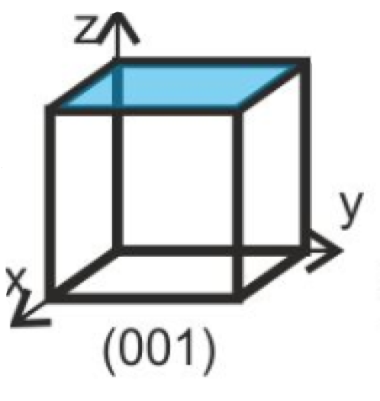
\includegraphics[scale = 0.4]{001.png}
            \caption{Stellt die (001)-Ebene graphisch dar.[1]}
            \label{A1}
        \end{minipage}
        \hfill
        \begin{minipage}[t]{0.45\linewidth}
            \centering
            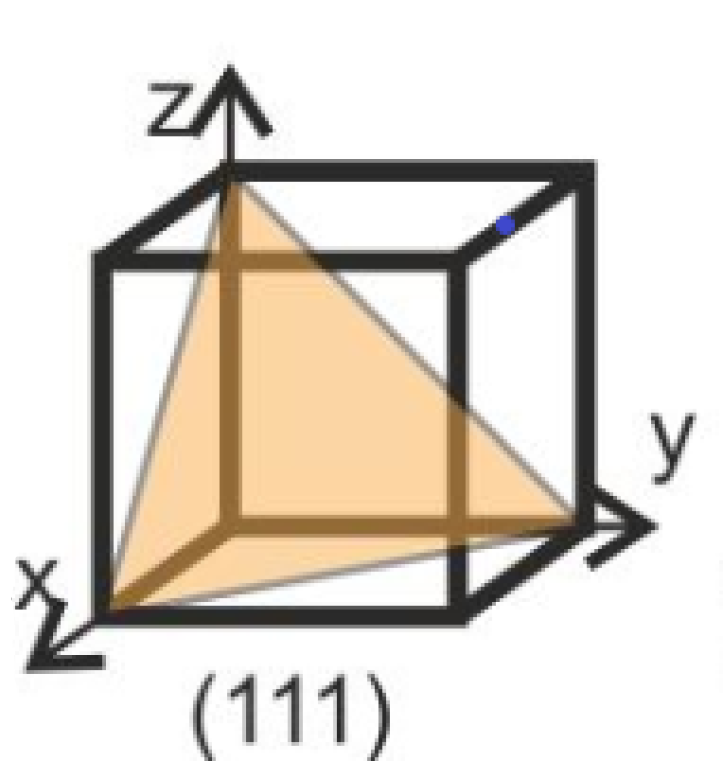
\includegraphics[scale = 0.25]{111.png}
            \caption{Stellt die (111)-Ebene graphisch dar.[1]}
            \label{A2}
        \end{minipage}
\end{figure}
Der (001) Reflex ist ein Überstrukturreflex und wächst bei zunehmender Ordnung, wohingegen der (111) Reflex ein Fundamentalreflex ist und sich mit längerer Wartedauer am Phasenübergang nicht ändert. Das Ziel dieses Abschnitts des Berichts ist es herauszufinden, wie sich der Ordnungsparameter ändert. Dazu wird der Ordnungsparameter $\eta$ gemäß des JMAK-Modells[2] eingeführt. \\
\begin{align}
    \eta^2 &= {\frac{I_\textsuperscript{exp}^{Ü}}{I_\textsuperscript{exp}^{F}}}
    \cdot 
    ({\frac{(f_\textsuperscript{Au}+3f_\textsuperscript{Cu})^{F}}{(f_\text{Au}-f_\textsuperscript{Cu})^{Ü}}})^{2}
    \cdot
    {\frac{p^{F}}{p^{Ü}}}
    \cdot
    {\frac{L_\textsuperscript{p}^{F}}{L_\textsuperscript{p}^{Ü}}}
    \cdot
    {\frac{D_\textsuperscript{T}^{F}}{D_\textsuperscript{T}^{Ü}}}
    \label{F1}
\end{align}
 Dabei sind die einzelnen Komponenten wie folgt definiert. Die Buchstaben "Ü" und "F" stehen für die jeweiligen Faktoren der Überstrukturreflexe bzw. der Fundamentalstrukturreflexe. Die Intensität des Überstrukturreflexes ist $I_\text{exp}^{Ü}$ und die Intensität des Fundamentalreflexes ist $I_\text{exp}^{F}$. Diese werden aus den Messungen abgelesen.
 Die Atomformfaktoren sind $f_\text{Au}$ und $f_\text{Cu}$. Diese sind für die Überstrukturreflexe und die Fundamentalreflexen identisch. Sie berücksichtigen die Lage der Atome in einer Elementarzelle. Um die Formfaktoren zu berechnen, benötigt man Parameter $a_i$,$b_i$ und $c$. Diese werden aus [2] entnommen.
 Der Flächenhäufungsfaktor $p$ berücksichtigt, wie häufig die einzelnen Netzebenen vorkommen. 
 Durch den Lorentz-Polarisationsfaktor $L_\text{p}$ werden geometrische Effekte der Röntenstrahlung korrigiert.
 Mit dem Debye- Waller-Faktor $D_\text{T}$ wird der Einfluss der Wärmebewegung berücksichtigt. Hierfür muss eine Konstante $B$ ermittelt werden, die für 400°C $B = 1,6187$ ist.
 Die jeweiligen Faktoren wurden, wie in [2] angegeben, berechnet. 
 \begin{align}
     f_\textsuperscript{Atom} &= \sum_{i=0}^N a_i\exp{(-b_is^2)} +c
 \end{align}
 \begin{align}
     p_\textsuperscript{(001)} &= 6 \\
     p_\textsuperscript{(001)} &= 8
 \end{align}
\begin{align}
    L_\textsuperscript{p} = \frac{1+\cos{2\theta}^2}{\sin{\theta}^2\cdot\cos{\theta}}
\end{align}
\begin{align}
    D_\textsuperscript{T} &= \exp{(-2B\frac{\sin{\theta}^2}{\lambda^2})} \\
    B &= 1,6187
\end{align}
Als letzten Aspekt wurde der Fernordnungsparameter auf die Zeit aufgetragen, um zu beschreiben, wie sich die Dynamik von $\eta$ verhält. Nach dem JMAK-Modell soll die zeitliche Veränderung beschrieben werden durch eine Konstante $k$, die von der Nukleationsrate und der Wachstumsgeschwindigkeit der Keime abhängig ist, und dem Avrami-Exponenten $n$.
\begin{align}
    \eta(t) = 1- exp(-kt^n)
\end{align}
Dabei wird überprüft, ob der theoretische Wert von $\eta = 4$ angenommen wird.

\subsection{Auswertung}
Als erstes wird die Dynamik des (001) Überstrukturreflex analysiert. Die erste und die zweite Messung sind vom Rauschen überzogen, sodass nicht erkannt werden kann, ob überhaupt ein Reflex auftaucht. Mit der Zeit bildet sich ein Peak aus, welcher sich vom Rauschen abhebt. Ab der 15. Messung ist zu sehen, dass sich ein Überstrukturreflex gebildet hat.
\begin{figure}[h!]
    \centering
    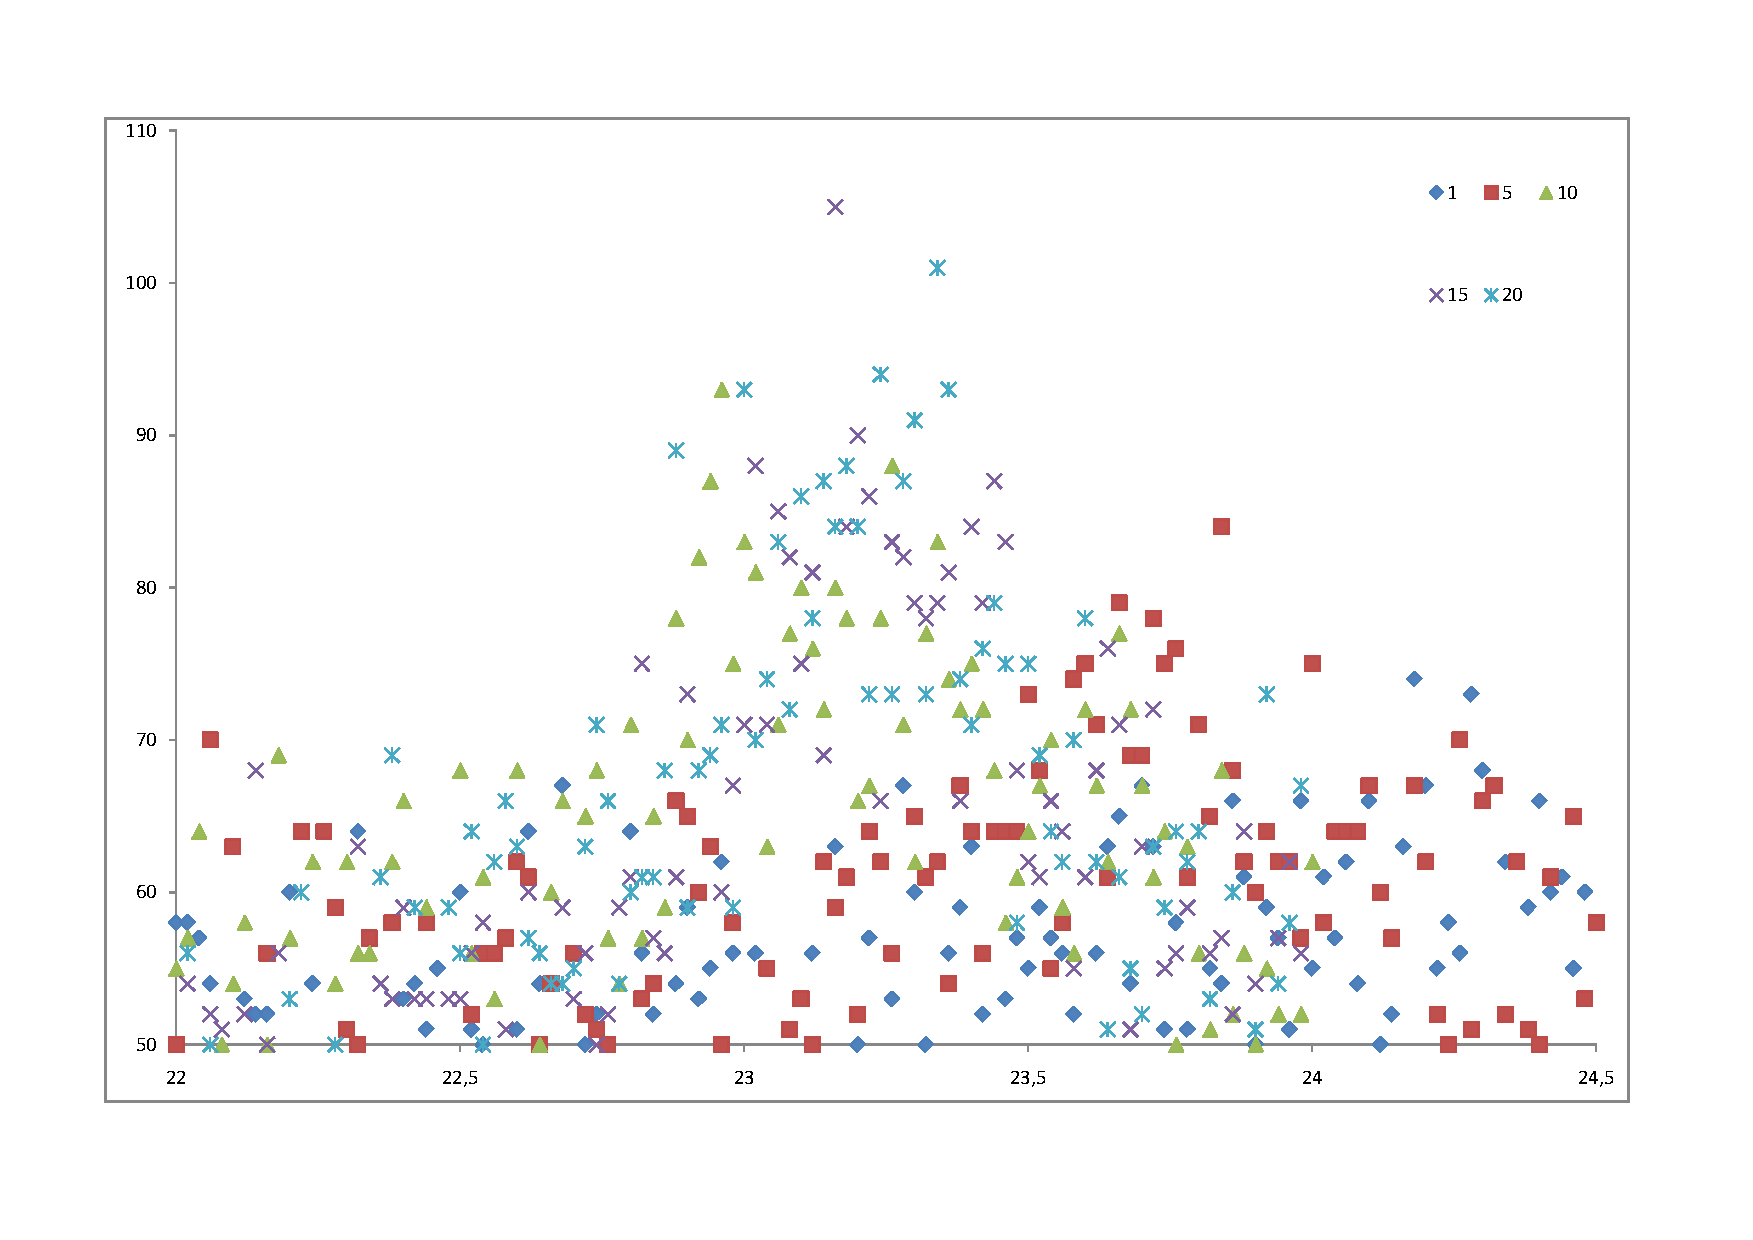
\includegraphics[scale = 0.5]{Bragg_Punkte.pdf}
    \caption{Diese Graphik stellt die Dynamik (001)-Ebene dar. Auf der $x$-Achse ist der Winkel in Grad und auf der $y$-Achse die Intensität der einfallenden Röntenstrahlung angegeben. Die dunkelblauen Rauten sind die ersten Messungen, die roten Quadrate die Fünften, die grünen Dreiecke die Zehnten, die violetten Kreuze die Fünfzehnten und die hellblauen Kreuze die Zwanzigsten.}
    \label{A3}
\end{figure}
Anhand von \cref{A3} konnte beobachtet werden, dass sich innerhalb der Messwerte nach der 15. Messung nicht mehr viel in der Dynamik abgespielt hat, sodass dies als neue Phase erkannt wurde. Durch diesen stationären Zustand kann der Ordnungsgrad ermittelt werden. Dieser lag bei kleinen Temperaturen (25°C) bei $\eta = 1$ und bei hohen Temperaturen(x > 700°C) bei $\eta = 0$. Da $\eta$ ein Maß der Ordnung darstellt und dies gerade das Verhältnis von dem (001) und (111) Reflex nach \cref{F1} ist, werden deren Größenordungen bei 400°C durch \cref{A3} veranschaulicht.
\begin{figure}[h!]
    \centering
    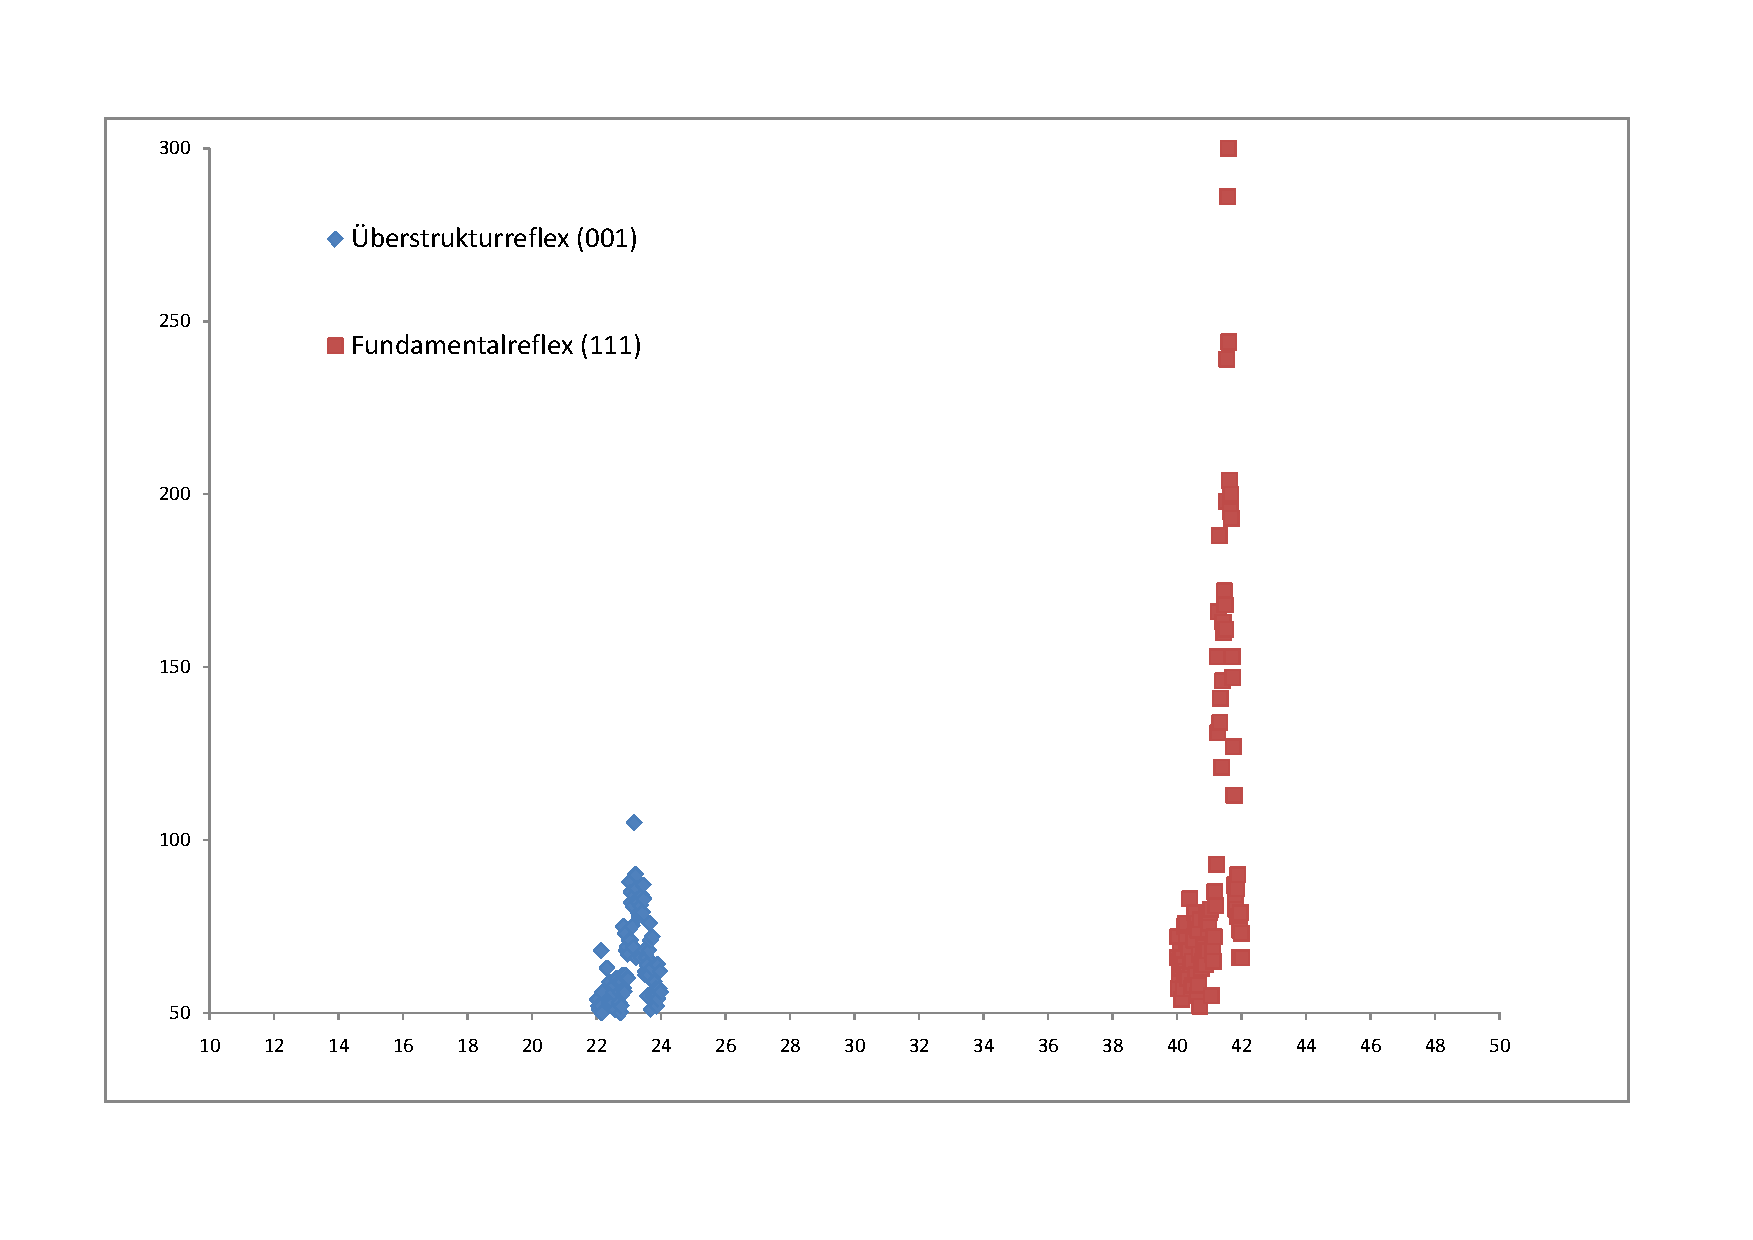
\includegraphics[scale = 0.5]{001 und 111.pdf}
    \caption{Diese Grafik stellt die (001) und die (111) Reflexe im stationären Zustand dar. Auf der $x$-Achse ist der Winkel in Grad und auf der $y$-Achse die Intensität der einfallenden Röntenstrahlung angegeben. Der Überstrukturreflex stellt die 15. Messung dar, wohingegen der Fundamentalreflex sich über die Zeit nicht geändert hat.}
    \label{A4}
\end{figure}
Der Überstrukturreflex ist die 15. Messung, die gemacht wurde. Diese Messung wurde zur bildlichen Darstellung benutzt, da diese den höchsten Wert innerhalb der Messreihe besessen hat. Während der Auswertung wurde jedoch mit allen Messwerten gerechnet.
Über Formel \cref{F1} wurden die Ordnungsparameter bestimmt. Dazu wurde beim (111) Reflex ein Mittelwert der beiden Referenzwerte genommen, um näher am statistischen Mittel zu liegen. Der (111) Wert hat sich mit der Zeit kaum geändert, sodass hier ein mit den variierenden Parametern zeitlicher konstanter Peak angenommen wurde. Um ein Mittel bzgl. dieser beiden Messwerte zu benutzen wurde der Mittelwert betrachtet. In \cref{A4} können die Messpunkte betrachtet werden. 
\begin{figure}[h!]
    \centering
    \includegraphics[scale = 0.7]{fit.png}
    \caption{Die Ordnung steigt mit zunehmender Zeit. Vor dem Anstieg hatte die Ordnung einen festen Wert. Nach dem Anstieg wird der Wert  ebenfalls auf einem Wert verharren, bis sich die Phase wieder ändert, sodass hier ein logistisches Wachstum der Ordnung angenommen werden kann. Hier ist nur der Ausschnitt des Wachstums dargestellt. Die Messunsicherheiten sind dabei so klein, dass sie nicht zu sehen sind. Der Fit wurde mit OriginPro berechnet.
    $\eta = 1 - exp(-kt^n)$ mit $k=0,32 \pm 0,02$ und $n=0,07 \pm 0,01$}
    \label{A5}
\end{figure}

Nun wurden die Ordnungsparameter berechnet und auf \cref{A5} dargestellt. Die Zeitbalken auf der $x$-Achse müssen nicht immer denselben Abstand haben. Diese Unsicherheit wurde im folgenden ignoriert. Dieser Graph zeigt wie sich die Ordnung beim Phasenübergang verhält. Vor dem Phasenübergang existierte eine stabile Ordnung. Dann wird die Ordnung bei der Phasenumwandlung so lange verändert, bis eine neue Ordnung entsteht, die wieder stabil ist. In \cref{A5} ist jedoch nur die Dynamik des Übergangs dargestellt. Anhand des Fits können folgende Parameter bestimmt werden. \\
$\eta = 1 - exp(-kt^n)$ mit $k=0,32 \pm 0,02$ und $n=0,07 \pm 0,01$\\
Hieraus kann abgelesen werden, dass der Avrami-Exponenten nicht den theoretischen Wert von n=4 angenommen hat.


\subsection{Unsicherheit}
Um die Unsicherheiten zu berechnen, wurde geschaut, welche Messungen die höchste Messunsicherheit hatte. Innerhalb unserer Messwerte konnte die größte Messunsicherheit der Intensitätsmessung zugewiesen werden, sodass diese durch eine Dreieckswahrscheinlichkeitsdichtefunktion abgeschätzt wurde. Alle anderen Messwerte wurden vernachlässigt, da diese zur Gesamtunsicherheit vernachlässigbar sind.
\begin{align*}
    u_{I_\textsuperscript{max}} &= \frac{1[I]}{2\sqrt{6}} &= 0,02[I]
\end{align*}
Die weiteren Rechnungen wurden mithilfe der Fehlerfortpflanzung ermittelt. Diese wurde nur bei den Termen angewandt, wo der größte Fehler aufgetreten ist.
\begin{align*}
    u_{\eta^2}^2 &= ({\frac{1}{I_\textsuperscript{exp}^{F}}}
    \cdot 
    ({\frac{(f_\textsuperscript{Au}+3f_\textsuperscript{Cu})^{F}}{(f_\textsuperscript{Au}-f_\textsuperscript{Cu})^{Ü}}})^{2}
    \cdot
    {\frac{p^{F}}{p^{Ü}}}
    \cdot
    {\frac{L_\textsuperscript{p}^{F}}{L_\textsuperscript{p}^{Ü}}}
    \cdot
    {\frac{D_\textsuperscript{T}^{F}}{D_\textsuperscript{T}^{Ü}}}u_{I_\textsuperscript{max}^{Ü}})^2 + 
    ({\frac{I_\textsuperscript{exp}^{Ü}}{I_\textsuperscript{exp}^{F^2}}}
    \cdot 
    ({\frac{(f_\textsuperscript{Au}+3f_\textsuperscript{Cu})^{F}}{(f_\textsuperscript{Au}-f_\textsuperscript{Cu})^{Ü}}})^{2}
    \cdot
    {\frac{p^{F}}{p^{Ü}}}
    \cdot
    {\frac{L_\textsuperscript{p}^{F}}{L_\textsuperscript{p}^{Ü}}}
    \cdot
    {\frac{D_\textsuperscript{T}^{F}}{D_\textsuperscript{T}^{Ü}}}u_{I_\textsuperscript{max}^{F}})^2
\end{align*}
Weitere Unsicherheiten wurden über den Fit bestimmt, der mit OriginPro berechnet wurde.


\subsection{Diskussion}
Innerhalb dieser Auswertung wurde eine Näherung für die Dynamik bei einem Phasenübergang gemacht. Da der (001) Reflex wieder auftaucht, kann darauf geschlossen werden, dass die Ordnung im Kristall zunimmt, da neue Symmetrien auftauchen. Anhand von \cref{A5} kann gesehen werden, dass die Ordnung zwischen (0,4-0,6) liegt. Dies entspricht unseren Erwartungen, da $0$ vollständiger Unordnung entsprach, wohingegen $1$ der vollständigen Ordnung entsprach. Da die Temperatur inmitten der zugeordneten Temperaturskala (25°C - 700°C) liegt, ist es logisch, dass auch der Ordnungsparameter etwa in der Mitte der Werte liegt. Das ein Anstieg zu begutachten ist, ist auch plausibel, da einmal der Phasenübergang eine zeitliche Entwicklung braucht, aber auch, weil von 400°C auf 375°C reduziert wurde. So könnte ein zeitlich Veränderliches $B$ (Debye-Waller-Faktor) zur genaueren Untersuchung dieses Sachverhaltes eingebaut werden. Der berechnete Fit stimmt jedoch zu der theoretischen Überlegung von n=4 nicht. In diesem Fall wurde n zu $n=0,07 \pm 0,01$ berechnet. Der Fehler liegt vermutlich im Fit. Es könnte sein, dass das Programm zu wenig variable Parameter besessen hatte, um die Messwerte gut genug abzubilden. So müsste ein Verschub in der Zeit, eine andere Amplitude oder ein Offset der Daten berücksichtigt werden, um näher am theoretischen Ergebnis zu landen. So ist die Gleichung vom JMAK-Modell nicht an experimentelle Messdaten angepasst, sodass an der zu fittenden Funktion eine Änderung vorgenommen werden müsste.

\newpage

\section{Kalorimetrie}
\subsection{Methoden und Durchführung}
Zur Analyse des Phasenübergangs in der CuAu-Legierung wird auch eine kalorimetrische Untersuchung durchgeführt. Hierfür wird ein dynamisches Wärmestromdifferenzkalorimeter, zu sehen in \cref{kalori}, verwendet. Mit diesem werden Temperaturdifferenzen zwischen einer Probe und einer Referenz gemessen, die sich beide in einem Aluminiumtiegel befinden. Die Differenz ist in diesem Versuch ein leerer Tiegel (Luftreferenz). Beide befinden sich dabei in einer Kammer, in der sie symmetrisch auf einer Scheibe positioniert werden. ("disk-type") Wenn die Kammer nun aufgeheizt wird, kann über die Scheibe die Temperaturdifferenz zwischen den beiden Proben ermittelt werden.

\begin{figure}[h]
	\centering
	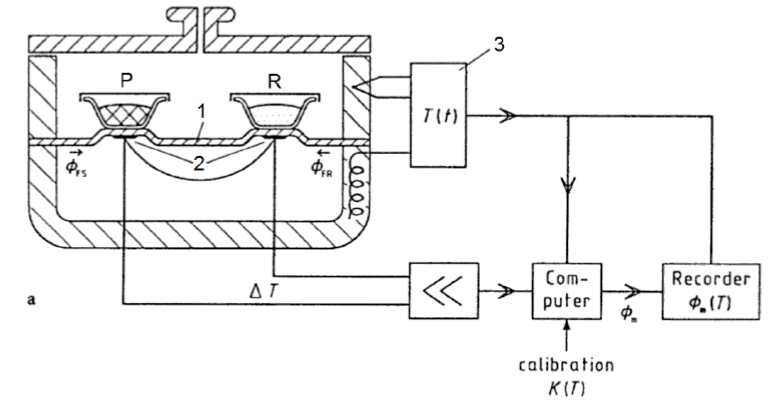
\includegraphics[scale=0.7]{Kalorimeter.png}
	\caption{Aufbau eines "disk-type" Wärmestrom-DSC. P: Probe, R: Referenz, 1: Scheibe,
		2: Thermoelemente, 3: Temperaturregelung. [2]}
	\label{kalori}
\end{figure}

Die Methode wird an dieser Stelle verwendet, um den Phasenübergang zwischen Ordnung und Unordnung in der CuAu-Legierung zu untersuchen. Hierfür wird die Kammer zuerst auf eine Temperatur von $\SI{500}{\degreeCelsius}$ gebracht. Diese liegt deutlich über der Phasenübergangstemperatur, deswegen ist der Kristall in diesem Zustand ungeordnet. Anschließend wird die Kammer wieder abgekühlt, zuerst auf $\SI{410}{\degreeCelsius}$ mit einer Rate von $\SI{60}{\degreeCelsius/\minute}$, anschließend sehr langsam mit einer Rate von $\SI{5}{\degreeCelsius/\minute}$ auf $\SI{385}{\degreeCelsius}$. Diese Temperatur liegt knapp unterhalb der Phasenübergangstemperatur von $\SI{390}{\degreeCelsius}$, daher ist nun der Phasenübergang der Legierung zu erwarten. Um diesen zu beobachten, wird die Temperatur nun für $\SI{30}{\minute}$ konstant gehalten. Der Phasenübergang von Unordnung zu Ordnung ist ein exothermer Vorgang, das heißt die Probe gibt dabei Wärme ab. Dieser Wärmefluss kann über die Temperaturdifferenz bestimmt werden. Da der Wärmefluss ein Maß für die Änderung des umgewandelten Volumens im isothermen Phasenübergang ist, kann mit diesem untersucht werden, inwiefern die Versuchsergebnisse mit der zeitlich abgeleiteten Johnson-Mehl-Avrami-Kolmogorow-Gleichung (\cref{eq:jmak}) übereinstimmen. Insbesondere soll betrachtet werden, ob die Wahl des Avrami-Exponenten auf $n=4$ mit den Messwerten übereinstimmt.
\begin{equation}
	\frac{\mathrm{d}X(t)}{\mathrm{d}t} = H \cdot K \cdot n \cdot \exp(-K\cdot (t-t_0)^n)\cdot (t-t_0)^{n-1}
	\label{eq:jmak}
\end{equation}

\subsection{Auswertung und Diskussion}
In \cref{3} wurde der im Kalorimeter gemessene Wärmestrom gegen die Zeit aufgetragen. Zuerst steigt der Wärmestrom sehr stark, das liegt daran, dass sich das System erst in der Isotherme einpendeln muss, da die Kammer vorher gekühlt wurde. Dieser Vorgang dauert etwa $105$ Sekunden, an dieser Stelle ist ein lokales Maximum erreicht. Anschließend sinkt der Wärmefluss wieder, erreicht nach ca. $300$ Sekunden ein lokales Minimum und steigt dann bis etwa $450$ Sekunden nach Beginn der Isotherme auf den Wert des vorherigen lokalen Maximums. Den Rest der Zeit steigt der Wärmefluss nur noch leicht an.

\begin{figure}[hb]
	\centering
	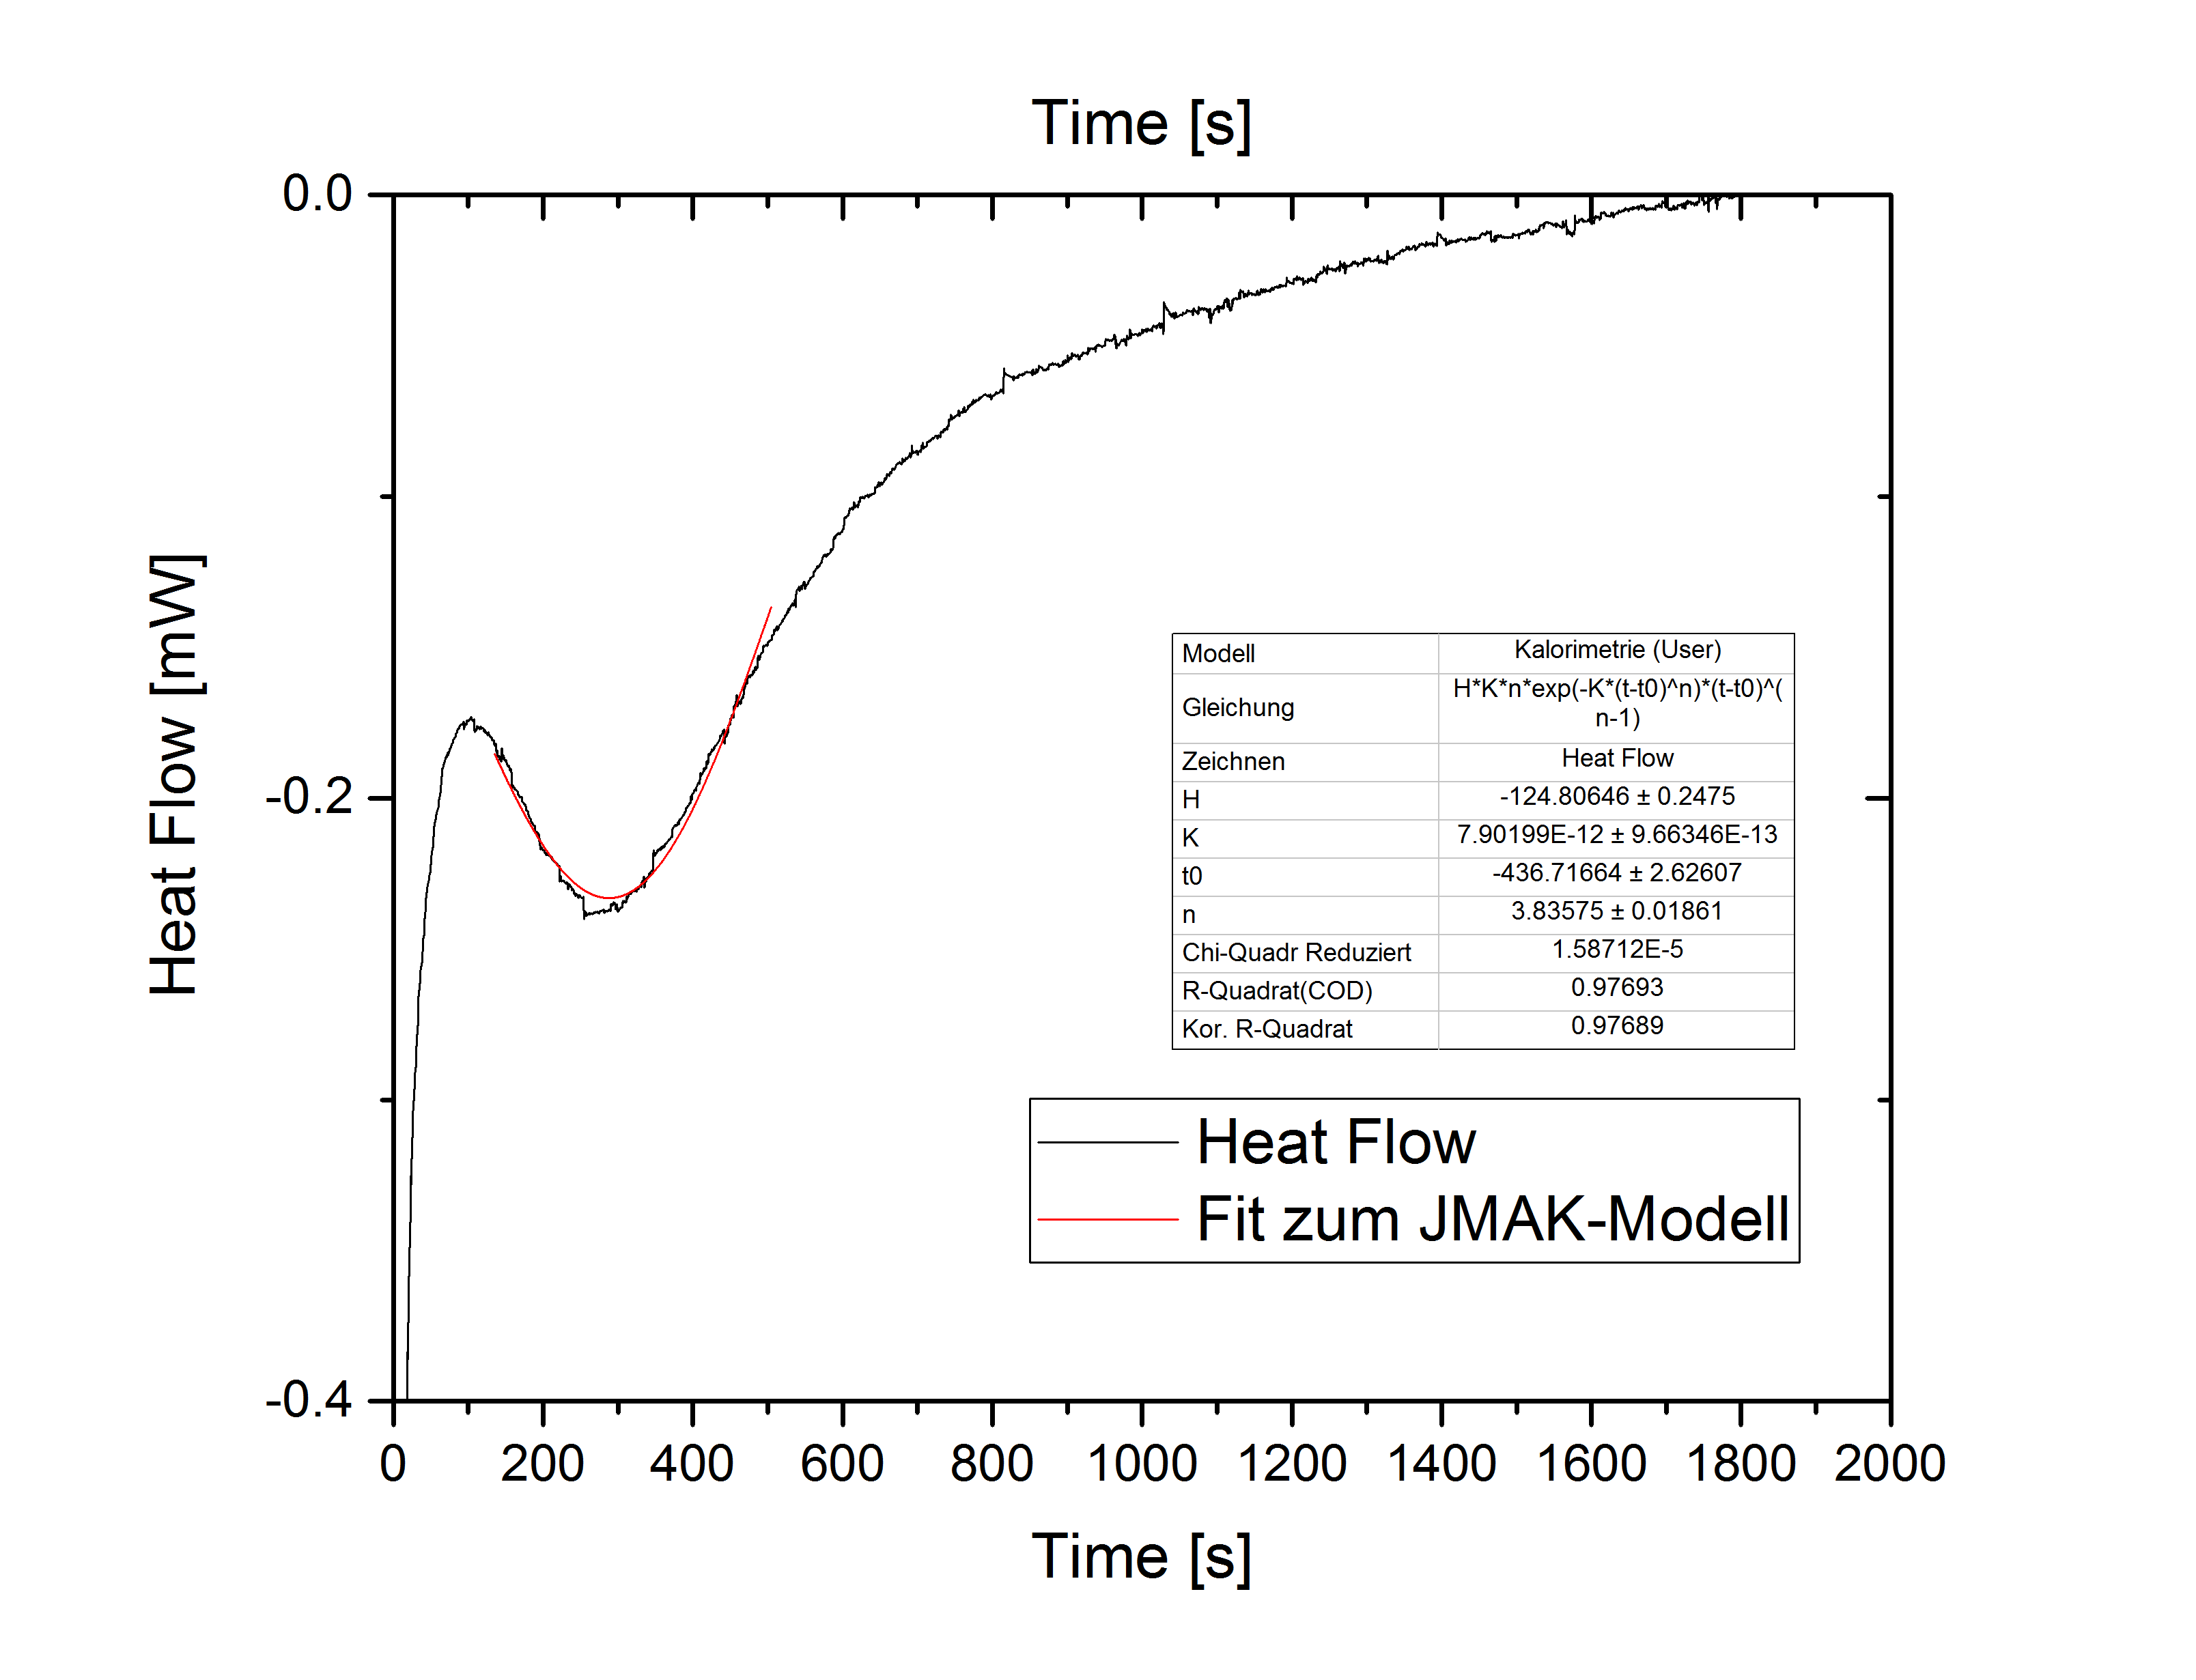
\includegraphics[scale=0.6]{Graph3.png}
	\caption{Der im Kalorimeter gemessene Wärmefluss aufgetragen gegen die Zeit und der an die Messwerte angepasste Fit nach dem JMAK-Modell}
	\label{3}
\end{figure}

Der Phasenübergang ist exotherm, währenddessen wird also Energie in Form von Wärme abgegeben. Dies äußert sich im Diagramm durch den nach unten zeigenden Peak im Intervall zwischen $105$ und $450$ Sekunden. In diesem Bereich findet der Phasenübergang zwischen Unordnung und Ordnung im Kristall statt. Der Phasenübergang startet zuerst langsam mit einem geringen Wärmefluss, vollzieht sich anschließend immer schneller, bis zeitlich nach der Hälfte des Übergangs der größte Wärmefluss erreicht wird. Anschließend wird der Vorgang wieder langsamer. Auf den Bereich des Phasenübergangs wird nun der Fit nach \cref{eq:jmak} angewendet. In der Formel wurden im Vergleich zur Anleitung einige Änderungen vorgenommen. Zum einen wurden die Parameter $H$ und $t_0$ ergänzt, zum anderen wurden alle Messwerte um $\SI{0,25}{mW}$ nach unten verschoben, da die angefittete Funktion nur im negativen Wertebereich definiert ist. Somit ergibt sich die in \cref{3} dargestellte Fitfunktion mit den angegebenen Parametern. Für $n$ wurde ein Wert von $3,84\pm0,02$ ermittelt. Der theoretisch vorhergesagte Wert liegt damit nicht innerhalb der angegebenen Unsicherheit.

Eine mögliche Ursache dafür liegt in der Form der untersuchten Probe. Nach dem JMAK-Modell setzt sich der Exponent der Exponentialfunktion vor allem aus zwei Faktoren zusammen. Erstens, dem Faktor $N\cdot t$, über den die Anzahl der Kerne in die Rechnung einfließt, zweitens dem Faktor $g \cdot t$, der die Ausbreitung der Körner in eine Raumrichtung beschreibt. Da der zweite Faktor in der Theorie für alle drei Raumrichtungen auftritt, ergibt sich damit der Exponent $n=4$. Die untersuchte Probe war allerdings sehr schmal, daher breiten sich die Körner vor allem in zwei Raumrichtungen aus, in die Dritte nicht so stark. Dies könnte erklären, dass der Exponent etwas kleiner ist als erwartet.

\newpage

\begin{thebibliography}{9}
\bibitem{A}
 \url{https://www.researchgate.net/figure/Miller-indices-indicating-the-plane-perpendicular-to-the-vector-given-for-the-cubic_fig7_302838100}\\
\bibitem{B}
Charakterisierung der Phasenumwandlung in Kupfer-Gold Legierungen,Fortgeschrittenen Praktikum, Versuchsanleitung, Münster ,WS 18/19

\end{thebibliography}
\end{document}
